\section{Getting Started}
\label{sec:iumlb-gettingstarted}

Since iUML-B diagrams are contained within Event-B machines, start by creating an Event-B project containing a Machine project. 
Then select the machine in the Event-B navigator and right click to use the context manual. 
The context manual contains commands to add the various kinds of iUML-B diagram to the machine.

Once the machine contains a diagram, it will appear in the Event-B navigator as an element within the machine.
To open the diagram for editing, double click on the iUML-B element in the Event-B navigator.

You can now use the diagram editor palette to create new elements on the canvas. 
Use the properties sheet to edit the detailed properties of an element.
Refer to the diagram specific user manuals within this manual.

Once the diagram model has been entered, the toolbar buttons can be used to process it.
The validate button (tick icon) runs a diagram validation test to check that the diagram is well-formed.
This validation is also performed automatically before you generate from the diagram.
To generate Event-B use the translate button (UML-B icon). 
The rules for generation of Event-B are given in the diagram specific manuals.

There is also a command (`Translate All iUML-B Diagrams') in the context manual of the machine (right click the machine in the Event-B navigator).
This translates all of the iUML-B diagrams contained in the machine.

\begin{figure}[!htbp]
	\centering
	\ifplastex
	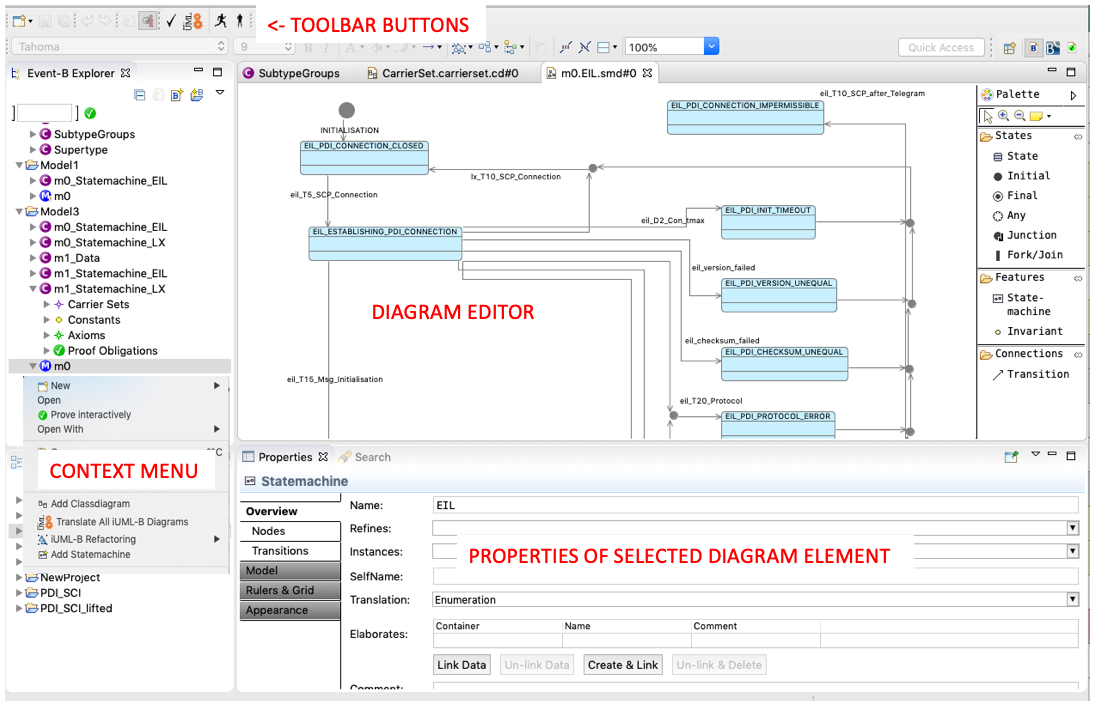
\includegraphics[width=1000]{figures/UMLB_UI.png}
	\else
	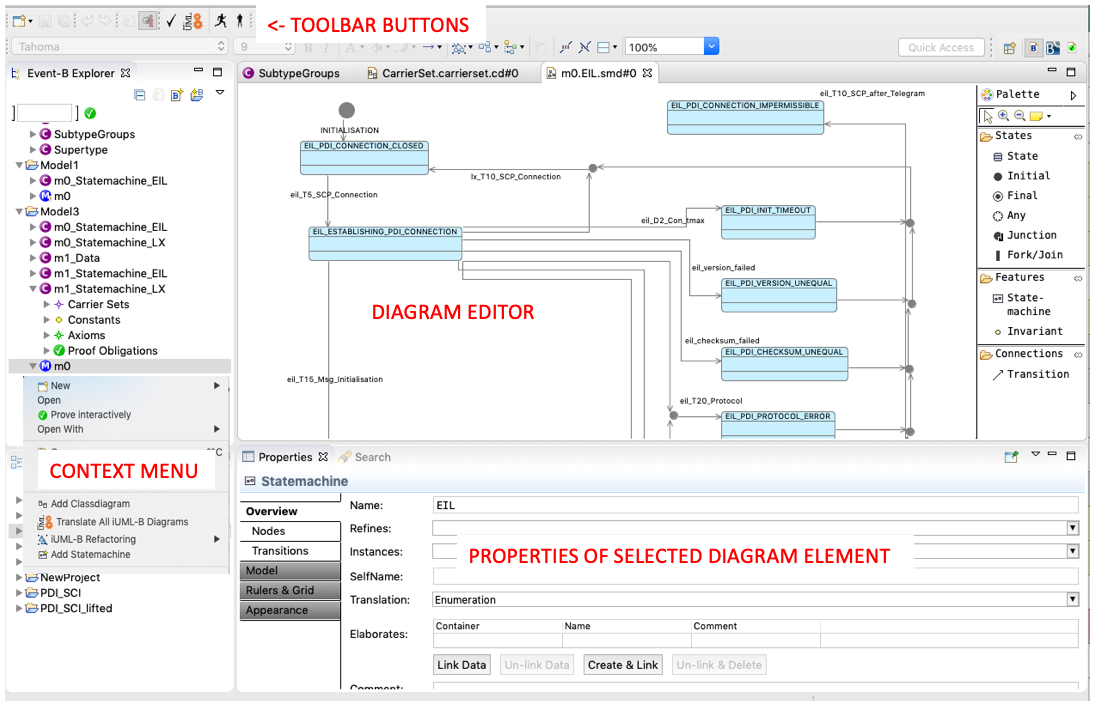
\includegraphics[width=1\textwidth]{figures/UMLB_UI.png}
	\fi
	\caption{User Interface for iUML-B}
	\label{fig:UMLB_UI}
\end{figure}